\section{Implementation and Methodologies}

This project had two major implementations, the annotator and the ML model,
which will be detailed in this chapter. The following will explain used
methodologies and choices made in the implementation process as well as overcome
difficulties. 

\subsection{Image-Annotator}

The purpose of the image annotation software is to give an easy possibility of
labeling, rescaling, cropping and saving images in order to be used as dataset
by the ML model.
\newline
The software was completely written in python, an interpreted script language.
Still python has object oriented features, that where partly used in this
project. 
\newline
The program program is structured in a way, to have two different classes,
"Window" and "popupWindow" to take care of the UI part of the project. The rest
of the functionality is structured into script-like functions. This structuring
makes it easier to split the program into smaller tasks that can be distributed
and worked on individually. This is a methodology oriented at the MVC (Model
View Controller) software development pattern. The UI is here clearly separated
from the controlling instance, that handles the backend of user interaction as
well as the model, which is responsible for data storage and maintenance. As
this is a simple single instance application, of course a detailed
implementation was not necessary and the model and controller are somewhat mixed
and both just represented as the separate functions. Still it gives the
possibility of separating the implementation of the UI, the backend and the
storage system.
\newline
The UI is handled by the the tkinter python library, which gives a lot of basic
functionality to easily implement the frontend of the application. The UI of
this project was mainly focused on the menu bar on top in addition to a
right-click menu. This choice was made in order to keep the overall frame clean
and focused on the most important thing, the image.
\newline
The backend storage uses a python dictionary to at all time store all edits made
by the software. If need be, the entirety of the data can be saved to file using
the JSON format and loaded back from it as well. To keep the storage as
efficient as possible and maintain the possibility to easily change categories,
they are saved separately with a second array only linking the index of
the annotation to the index of a category. Listing 1 shows a reduced example of
stored annotations. There is a feature enabling the user to save every processed
resized image to a specified location. It was disabled as it turned out not to
be needed in this project. 

\lstinputlisting[language=json,firstnumber=1,breaklines,caption={reduced example of saved annotations},captionpos=b]{../code/annotations.json}

The helping features are implemented as functions, that can be called through
the given menus:

\begin{description}[font=\sffamily\bfseries, leftmargin=1cm, style=nextline]
    \item[open image]
        Opens a file selector to let you chose an image to annotate
    \item[load next image]
        Finds the next image after natural order (the windows file-name order) in
        the same folder as the currently loaded image
    \item[save/import/view annotations]
        Lets the user chose a file location to either import or export all
        annotations as well as gives the possibility of viewing all currently
        loaded annotations in a list-view
    \item[add/replace/show category]
         Lets the user add a new category, replace an existing one or show all
         current categories in a list
    \item[import/export categories]
        Similar to annotations this gives the possibility to only share the
        categories by enabling exporting to json, csv or xlsx and importing from
        json and csv
    \item[replace/change destination]
        A feature that was not used during this project enabling the user to
        save each image resized and as png but not cropped to a specified
        location, that can be different for each image
\end{description}

Finally the main features of the annotation lay all in event listeners for the
mouse pointer. The user is able to draw rectangles in case an image was loaded.
A rectangle is only allowed if it has an area greater that 40 pixels, sides
longer than 5 pixels and is not overlapping with another rectangle by more than
20\%. Is a valid rectangle drawn, the user gets pointed details and is able to
chose a label. Figure \ref{fig:anno} shows the annotator in action. By
double-clicking or right-clicking the rectangle, this popup can be shown again
at any time and the label changed. Right-clicking also gives the choice of
deleting the rectangle.
\begin{figure}
    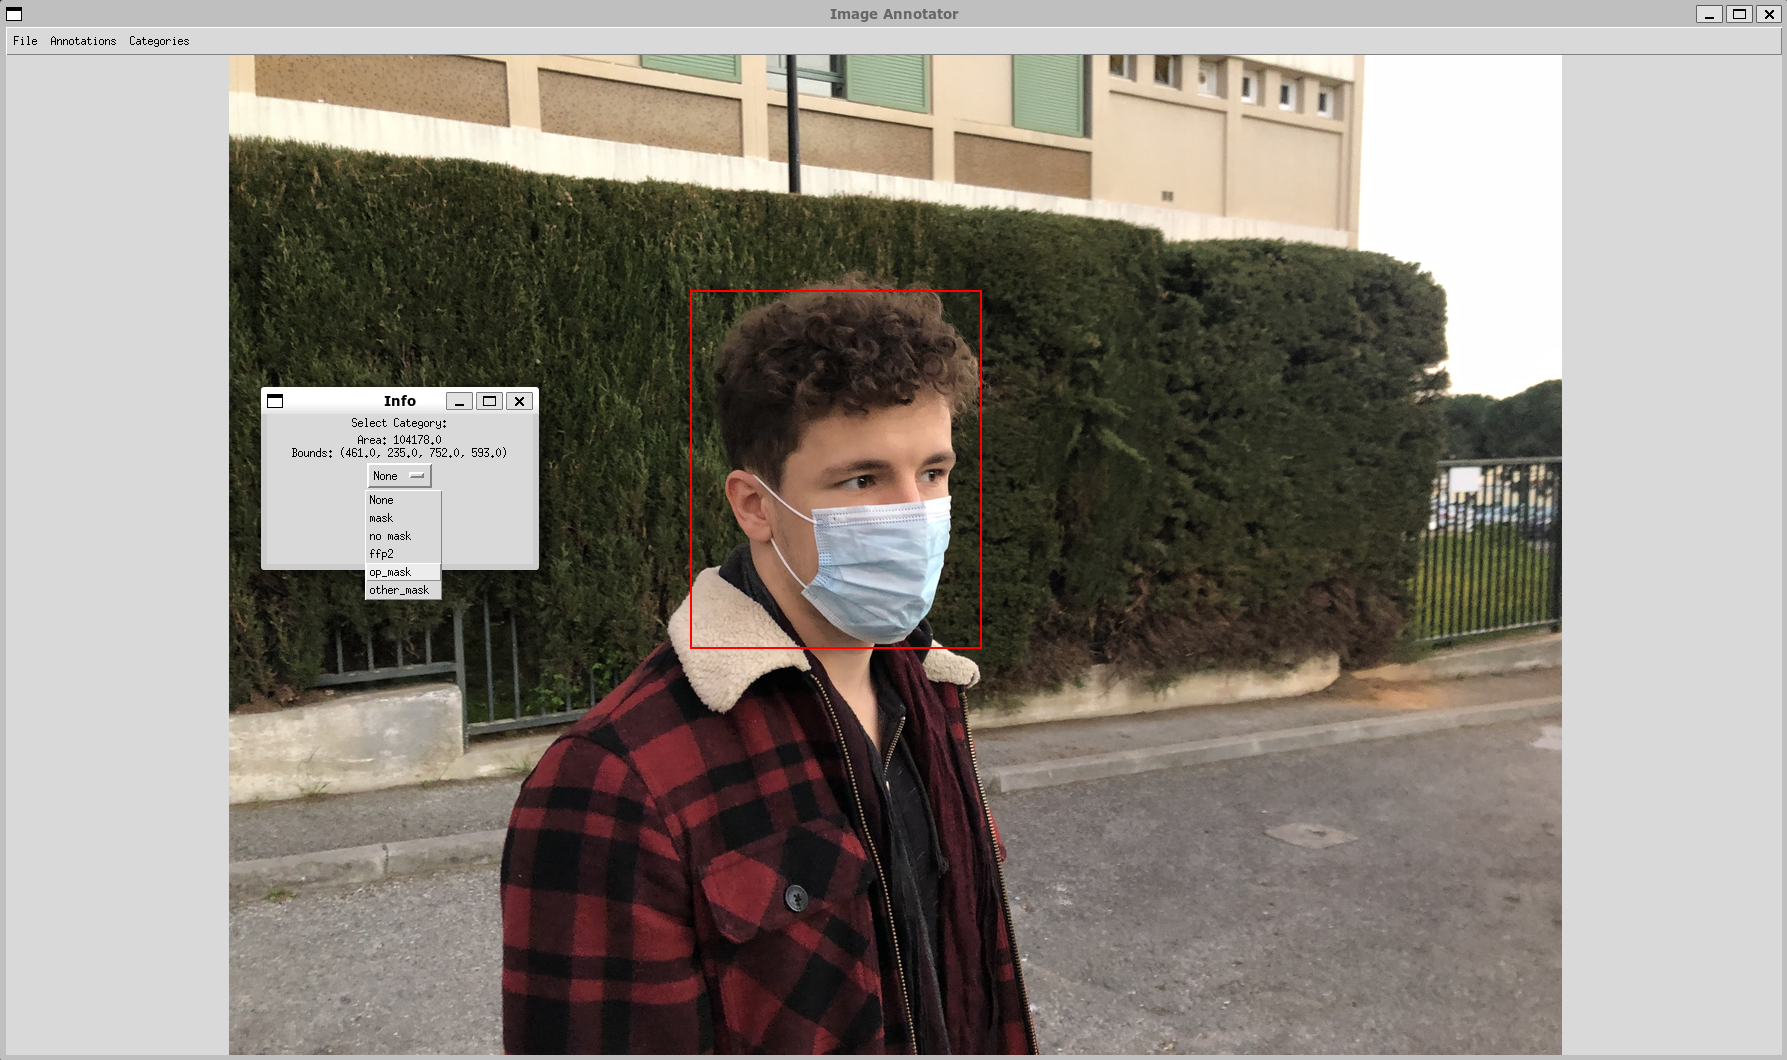
\includegraphics[width=\textwidth]{annotator_in_action.png}
    \caption{image annotator in action}
    \label{fig:anno}
\end{figure}
\newline
This gives the annotator the full needed functionality and enables a quick and
easy labeling of all the images. Once the labeling is done, the menu item
"\textbf{crop and save}" reloads each image at a time, crops all made rectangles
to 240x240 square format and saves them in folders according to their labeling
in an by the user specified location.

\subsection{Machine Learning Model}